\section{Introduction}
In recent years there has been a convergence between the fields of machine learning and discrete optimization, driven by the need to scale decision-making to increasingly complex problems. A wide body of research now investigates how learning-based models can complement or replace traditional algorithmic components in integer linear programming (ILP) pipelines, from branching strategies to primal heuristics and feasibility prediction. In parallel, energy-based models and graphical inference methods have been explored both as a way of solving optimization problems and as differentiable operations that can be included into machine learning models and aid in predicting structured solutions. Herein lies the main challenge that we aim to tackle through this thesis; predicting a feasible solution, that is an assignment that verifies the constraints of the problem. 

This chapter provides a structured overview of these developments. We first examine general-purpose and problem-specific learning approaches designed to enhance ILP solvers. We then review energy-based formulations of combinatorial problems, distinguishing between inference-driven techniques and learning-based energy models. By synthesizing these research directions, we highlight common principles, identify methodological gaps, and motivate the framework proposed in the subsequent chapters.

The central difficulty in applying machine learning to ILPs lies in the \emph{structured} nature of the prediction task. Unlike standard ML settings—such as classification or regression—where outputs have simple, low-dimensional forms (e.g., a probability vector over labels), ILP solutions are high-dimensional combinatorial objects whose components are tightly coupled through feasibility constraints. Predicting an ILP solution therefore requires producing not just accurate variable assignments, but assignments that jointly satisfy a rich set of constraints: connectivity in paths, disjointness in cuts, clique or independence relations in graphs, and more generally, global consistency enforced by the constraints. This sharply distinguishes ILP prediction from conventional learning tasks and aligns it more closely with structured prediction in graphical models, where the challenge is to ensure coherence across many interdependent variables.
The literature addresses this difficulty in several ways. Some approaches use post-processing mechanisms that \emph{project} an unconstrained prediction back onto the feasible set \cite{fischetti_feasibility_2005}; others temporarily embed the problem in a continuous latent space where differentiable learning is tractable, before mapping the resulting representation to a valid discrete solution. Broadly, existing ML-based methods fall into two categories. The first aims at general-purpose ILP solving by enhancing traditional branch-and-bound pipelines, learning policies for branching, pruning, or node selection to accelerate exact enumeration. The second group focuses on \emph{problem-specific} learning, where the model leverages properties of a particular combinatorial family—such as graph motifs or structure induced by the constraints—to directly predict coherent, feasible solutions.

In the remainder of this section, we provide an overview of these approaches. We begin with the extensive literature on \emph{learning to branch}, which offers foundational ideas and tools relevant to our setting. We then turn to generative methods that view ILP solutions through the lens of energy-based models, framing combinatorial optimization as probabilistic inference and enabling learned or amortized solution generation.

\section{Machine Learning for Integer Linear Programming}
In this section, we provide an overview of approaches that combine machine learning with standard methods for solving integer linear programs, with a particular focus on the Branch-and-Bound algorithm. Branch-and-Bound is a sophisticated enumeration framework that relies on a variety of heuristics to guide the search process. Many of the methods reviewed here aim to replace specific heuristic decisions with data-driven predictions, such as selecting the next branching variable or determining how the search space should be partitioned. It has been shown that the performance of enumeration-based solvers is highly sensitive to these heuristic choices. As a result, learning-based replacements can lead to substantial performance improvements while preserving the generality and exactness of the underlying algorithm, since worst-case guarantees remain unchanged.

More recently, problem-specific learning approaches have emerged for particular classes of combinatorial optimization problems. In these settings, optimization solvers often play the role of a structured component within a larger machine learning pipeline, for instance through learned greedy policies or black-box predictive models coupled with combinatorial solvers. Together, these lines of work illustrate a growing effort to integrate data-driven decision rules into both the internal mechanisms of general-purpose ILP solvers and the design of specialized learning-based optimization systems.

The literature on machine learning for combinatorial optimization is broad and rapidly evolving. While no survey focuses exclusively on individual solver components, many of the approaches discussed in this section are covered in general reviews of learning-augmented combinatorial optimization and MILP solvers, notably \cite{bengio_machine_2018} and \cite{cappart_combinatorial_2023}.

\subsection{General-Purpose Learning Frameworks for ILP}
General-purpose learning frameworks for ILPs focus on enhancing solver behavior in a problem-agnostic manner by learning data-driven policies for core decisions within branch-and-bound. Rather than tailoring models to specific problem structures, these approaches aim to generalize across diverse instances by operating directly on solver states. Central directions include learning branching and node selection policies, as well as auxiliary predictions such as feasibility, optimality, or instance difficulty, which can be integrated into the solver to guide search and accelerate convergence. Collectively, these methods define a class of learning-enhanced solvers that improve performance while retaining the generality and exactness of classical ILP algorithms.
 
\subsubsection{Learning to Branch in Branch-and-Bound}
Learning to branch encompasses a family of approaches that use machine learning to guide enumeration in branch-and-bound solvers. While all methods aim to evaluate the potential impact of decisions made during search, they differ in the locality of the learned signal, ranging from fine-grained variable selection policies to more global assessments that guide pruning, decomposition, or search-space partitioning. We organize this literature according to this distinction. Figure~\ref{fig:problem_agnostic_learning} summarizes the main ways learned models are integrated into branch-and-bound solvers by mapping solver states to decisions that control standard components of the search.

\begin{figure}[htbp]
\centering
\resizebox{0.9\textwidth}{!}{
\begin{tikzpicture}[
    node distance=1.2cm and 2.0cm,
    box/.style={draw, rounded corners, minimum width=3.1cm, minimum height=0.95cm, align=center, font=\small},
    group/.style={draw, rounded corners, inner sep=7pt, densely dashed},
    arrow/.style={-Latex, thick},
    flow/.style={-Latex, thick},
    info/.style={-Latex, dashed, thick},
]

% --- Left: different ILP problem families / distributions ---
\node[box] (scp) {SCP instances};
\node[box, above=of scp] (mis) {MIS instances};
\node[box, below=of scp] (vrp) {VRP, etc.};

\node[group, fit=(mis) (scp) (vrp), label=left:{\small Training / test distributions}] (problemgroup) {};

% --- Center: generic solver state extracted during B\&B ---
\node[box, right=1.6cm of scp, fill=gray!15] (state)
{Solver state\\{\scriptsize LP relaxation, bounds, incumbents, graph features}};

\draw[flow] (mis.east) -- (state.west);
\draw[flow] (scp.east) -- (state.west);
\draw[flow] (vrp.east) -- (state.west);

% --- Learned model ---
\node[box, right=1.6cm of state, fill=blue!10] (model)
{Learned decision model\\{\scriptsize imitation / RL / scoring}};

\draw[flow] (state.east) -- (model.west);

% --- Right: solver decisions controlled by the model ---
\node[box, right=1.8cm of model, fill=green!10] (branch)
{Branching\\(variable selection)};
\node[box, above=of branch, fill=green!10] (node)
{Node selection\\(prioritization)};
\node[box, below=of branch, fill=green!10] (cuts)
{Cut selection/\\ scheduling};
\node[box, below=of cuts, fill=green!10] (heur)
{Primal heuristics\\(diving / repair)};
\node[box, above=of node, fill=green!10] (restart)
{Restart / search\\strategy};

\node[group, fit=(restart) (node) (branch) (cuts) (heur),
      label=right:{\small Decision points in B\&B}] (decisiongroup) {};

% Arrows from model to decisions
\draw[arrow] (model.east) -- (branch.west);
\draw[arrow] (model.east) |- (node.west);
\draw[arrow] (model.east) |- (cuts.west);
\draw[arrow] (model.east) |- (heur.west);
\draw[arrow] (model.east) |- (restart.west);

% Feedback loop: decisions update solver state
\draw[info] (branch.south) |- ([xshift=0.0cm]state.south);
\draw[info] (node.south)   |- ([xshift=-0.3cm]state.south);
\draw[info] (cuts.south)   |- ([xshift=0.3cm]state.south);

\node[font=\scriptsize, align=center, below=0.6cm of model] (looptext)
{Decisions update the search tree and constraints\\and therefore change subsequent solver states};

\end{tikzpicture}
}

\caption{Overview of learning-augmented branch-and-bound. Across different ILP instance distributions, solver states encountered during enumeration are encoded and passed to a learned decision model (e.g., imitation learning, reinforcement learning, or learned scoring). The model outputs decisions for standard solver components such as branching, node selection, cut management, primal heuristics, and restart strategies. These decisions in turn modify the search process, creating a feedback loop through the evolving solver state.}
\label{fig:problem_agnostic_learning}
\end{figure}


\paragraph{Local decision learning: branching policies.} Branching is one of the most influential local decisions in branch-and-bound (B\&B), as it directly determines the size and structure of the search tree. Classical branching rules rely on handcrafted heuristics such as strong branching, pseudocost branching, and reliability branching \cite{achterberg_constraint_2007}. Learning to branch aims to replace or augment these heuristics with data-driven policies that evaluate the immediate impact of candidate branching actions.
Early work by Khalil et al.\ \cite{khalil_learning_2016} framed branching as a supervised learning problem, using engineered features to predict strong branching scores and guide variable selection. This line of work established the feasibility of learning branching policies that generalize across instances while remaining compatible with exact solvers.
A major step toward representation learning was introduced by Gasse et al.\ \cite{gasse_exact_2019}, who proposed a graph neural network that encodes the solver state as a bipartite variable–constraint graph and imitates strong branching decisions. This approach demonstrated that high-quality branching policies can be learned offline and transferred across instance distributions, and it has since become a reference architecture for learning-based branching.
Subsequent work explored reinforcement learning formulations of branching, treating variable selection as a sequential decision-making problem. Notably, He et al.\ \cite{he_learning_2014} and Nair et al.\ \cite{nair_solving_2020} optimize branching policies with respect to global solver objectives such as tree size or solution time, combining branching decisions with auxiliary mechanisms such as pruning. Hybrid approaches further integrate imitation learning, reinforcement learning, and handcrafted signals to improve stability and data efficiency \cite{khalil_learning_2016, ding_accelerating_2020}.
More recent contributions focus on improving generalization and interpretability. Wang et al.\ \cite{wang_learning_2024} propose a pointer-based architecture for variable selection that enables flexible attention over solver states, while Kuang et al.\ \cite{kuang_towards_2024} introduce a symbolic learning framework that discovers interpretable branching rules directly from bipartite graph representations. Collectively, these methods represent increasingly expressive yet solver-compatible approaches to learning local branching decisions.
Figure~\ref{fig:learning_to_branch} illustrates learning to branch as a local decision process, in which a learned policy selects branching actions based solely on the current node state and is re-applied independently at each step of the enumeration.

\begin{figure}[H]
\centering
\begin{forest}
for tree={
    draw,
    rounded corners,
    align=center,
    minimum width=2.6cm,
    minimum height=1cm,
    inner sep=4pt,
    font=\small,
    edge={-Latex}
},
selected/.style={fill=blue!10},
good/.style={fill=green!20},
bad/.style={fill=red!20},
local/.style={fill=yellow!15},
edge label/.style={midway, sloped, font=\scriptsize}
%
% ---------------- TREE ----------------
[Node $P_0$\\Local solver state\\{\scriptsize LP sol., bounds}
    [Branch on $x_i \le 0$, good,
        edge label={node[midway,above]{local policy}}
    ]
    [Branch on $x_i \ge 1$, selected,
        edge label={node[midway,above]{local policy}}
        [Node $P_1$\\Local solver state\\{\scriptsize LP sol., bounds}
            [Pruned, bad,
                edge label={node[midway,above]{bound}}
            ]
            [Feasible, good,
                edge label={node[midway,above]{solution}}
            ]
        ]
    ]
]
\end{forest}

% Local decision model
\vspace{0.4cm}
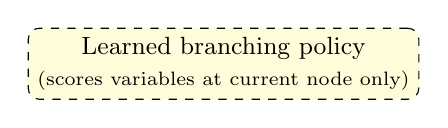
\begin{tikzpicture}
\node[draw, dashed, rounded corners, fill=yellow!15, font=\small, align=center]
{Learned branching policy\\{\scriptsize (scores variables at current node only)}};
\end{tikzpicture}

\caption{Local decision-making in learning to branch. A learned branching policy evaluates only the current node state to score candidate variables and select a branching action. The policy is re-applied independently at each node of the branch-and-bound tree, guiding local tree expansion without explicit evaluation of downstream subtrees.}
\label{fig:learning_to_branch}
\end{figure}


\paragraph{Global and semi-global branching guidance.} Beyond immediate branching actions, several works learn more global or semi-global signals that guide how the search space is explored. Rather than selecting a specific branching variable, these approaches evaluate the potential utility of nodes, subtrees, or structural transformations, and use these assessments to influence pruning, node prioritization, or solver strategy selection.
Some learning-to-branch methods incorporate global feedback directly into branching decisions. For instance, the lookback mechanism proposed by \cite{gupta_lookback_2022} augments local branching policies with information about downstream solver behavior, reducing the risk of missing decisions with delayed impact. Similarly, reinforcement learning approaches such as \cite{he_learning_2014} combine branching with learned pruning rules, blurring the boundary between local action selection and global search control.
Other works extend learning-based guidance beyond branching itself. In particular, \cite{salvagnin_learning_2017} studies the problem of learning when to invoke decomposition techniques during branch-and-bound, using learned predictors to assess structural properties such as decomposability or hardness. While operating at a coarser level than variable selection, these methods share the same underlying goal: learning surrogate measures of decision impact to guide enumeration more effectively.
Taken together, these approaches can be viewed as learning to branch at different levels of granularity. Local policies evaluate individual branching actions, while more global methods assess the expected utility of regions of the search space or solver interventions. Both perspectives contribute to a unified view of learning-guided branch-and-bound, in which learned models provide decision support across multiple scales of the search process.
As illustrated in Figure~\ref{fig:global_branching_guidance_fig}, global guidance methods operate by evaluating the potential of nodes or subtrees based on accumulated solver state, rather than selecting individual branching actions.

\begin{figure}[htbp]
\centering
\resizebox{0.9\textwidth}{!}{
\begin{tikzpicture}[
    node/.style={draw, rounded corners, minimum width=2.2cm, minimum height=0.95cm, align=center, font=\small},
    good/.style={fill=green!20},
    bad/.style={fill=red!20},
    undecided/.style={fill=blue!10},
    globalinfo/.style={fill=gray!15},
    edge/.style={-Latex, thick},
    info/.style={-Latex, dashed, thick}
]

% Root
\node[node, undecided] (root) {Node $P_0$\\Partial assign.};

% Global solver information
\node[node, globalinfo, below=1.4cm of root] (global) {Global solver state\\{\scriptsize bounds, incumbent, stats}};

% Level 1
\node[node, good, above left=1.2cm and 2.4cm of root] (n1) {Node $P_1$\\Utility\\{\scriptsize predicted HIGH}};
\node[node, bad, above right=1.2cm and 2.4cm of root] (n2) {Node $P_2$\\Utility\\{\scriptsize predicted LOW}};

% Level 2 (children of P1)
\node[node, good, above left=1.2cm and 1.3cm of n1] (n3) {Promising\\{\scriptsize keep / prioritize}};
\node[node, bad, above right=1.2cm and 1.3cm of n1] (n4) {Low potential\\{\scriptsize prune}};

% Tree edges (branching outcomes)
\draw[edge] (root) -- (n1);
\draw[edge] (root) -- (n2);
\draw[edge] (n1) -- (n3);
\draw[edge] (n1) -- (n4);

% Learned model box (fit around nodes it evaluates)
\node[draw, dashed, rounded corners, fit=(n1) (n2), inner sep=10pt,
      label=below:{\small Learned node utility model}] (modelbox) {};

% Information flow from global state to the learned model / evaluated nodes
\draw[info] (global) -- (root);
\draw[info] (global) -- (n1);
\draw[info] (global) -- (n2);

% Optional: show solver actions influenced by the model
\node[font=\scriptsize, right=0.8cm of n2] (prune1) {prune};
\draw[info] (n2.east) -- (prune1.west);

\node[font=\scriptsize, left=0.8cm of n3] (prio) {prioritize};
\draw[info] (n3.west) -- (prio.east);

\end{tikzpicture}}

\caption{Illustration of global and semi-global guidance during branch-and-bound. A learned node utility model evaluates partial subproblems using both the local node state and global solver information (e.g., bounds and incumbent statistics). The resulting utility estimates guide solver control decisions such as pruning and node prioritization, helping focus the search on promising regions of the tree.}
\label{fig:global_branching_guidance_fig}
\end{figure}


\paragraph{Global search control.} Beyond branching decisions themselves, a complementary stream of research studies learning-based strategies that guide branch-and-bound at a more global level, often independently of any specific ILP structure or problem family. Rather than predicting individual branching actions, these approaches aim to replace or augment generic solver components such as node selection, cut management, primal heuristics, restart policies, or scheduling rules with learned models that can transfer across heterogeneous combinatorial domains.
Several works focus on learning when and how to apply computationally expensive solver operations. For example, Balcan et al.\ \cite{balcan_learning_2024} propose learning-to-cut frameworks that predict effective cutting planes or determine when cut generation is likely to be beneficial, enabling adaptive control of solver effort without relying on problem-specific features. Similarly, Salvagnin et al.\ \cite{salvagnin_learning_2017} study learning when to invoke decomposition techniques, using learned signals to assess structural properties such as decomposability or expected problem hardness.
Other approaches learn global heuristics that influence the overall search trajectory. Neural diving and repair strategies, such as those explored by Nair et al.\ \cite{nair_solving_2020}, learn primal construction heuristics that generate high-quality partial assignments and warm starts that generalize across problem classes. More broadly, learning-based restart, scheduling, and solver-control policies have been proposed to dynamically adapt the global search strategy during enumeration \cite{battiti_learning_2017}.
Tang et al.\ \cite{tang_reinforcement_2020} propose a reinforcement learning framework for cut selection and show that their approach generalizes to larger instances than those seen during training, while outperforming user-designed heuristics.
Taken together, these methods extend learning-guided branch-and-bound beyond local branching decisions, demonstrating how learned models can provide global and semi-global guidance over the search process. By learning surrogate measures of decision utility at different levels of granularity, they contribute to a unified view of learning-enhanced solvers in which data-driven components complement classical optimization mechanisms throughout the search pipeline. For a recent survey of machine learning augmentation techniques for branch-and-bound, we refer the reader to \cite{scavuzzo_machine_2024}.


\subsection{Problem-Specific Learning Approaches}
Complementary to the general-purpose approaches discussed above, a substantial body of work considers learning approaches developed for individual families of combinatorial optimization problems. These problem-specific methods are typically constructed around the structural properties of a particular domain, such as graph connectivity patterns, coverage relations, or metric structure, and are trained on instances drawn from that problem class.
A defining feature of these approaches is the use of representations and learning mechanisms that are closely aligned with the semantics of the underlying optimization problem. Rather than relying on solver-agnostic features, models are often designed to reflect the natural variables, constraints, or solution structures of the domain under consideration. Learning is therefore guided by inductive biases that mirror known combinatorial properties, enabling the model to capture recurring patterns that arise within the problem family.
Because of this specialization, problem-specific learning frameworks are generally evaluated within a restricted setting and are not intended to transfer directly to unrelated optimization problems. Their primary objective is to leverage domain structure to inform decision-making or solution construction within a fixed class of instances. As such, they form a complementary strand of research that explores how machine learning can be integrated with combinatorial optimization when the problem structure is explicitly taken into account.


\subsubsection{Learning internal representations for solution construction}
A first class of problem-specific learning approaches focuses on learning internal representations of combinatorial problems that directly guide solution construction. In these methods, a model incrementally builds a solution by making a sequence of discrete decisions, such as selecting elements, ordering variables, or extending partial assignments. The learning objective is to map the current state of the problem and partial solution to the next action.
This paradigm has been widely explored in graph-based optimization problems, where graph neural networks are used to encode instance structure and propagate information relevant to feasibility, conflicts, or solution quality. Early work by Dai et al.~\cite{dai_learning_2017} demonstrated how reinforcement learning combined with message-passing architectures can learn greedy construction policies for problems such as Maximum Independent Set and Minimum Vertex Cover. Related approaches extend this idea to other graph problems, including Max-Cut and related formulations, often learning end-to-end policies or local search operators adapted to the combinatorial structure \cite{li_combinatorial_2018}.
Sequential construction models have also been developed for routing and sequencing problems, where solutions naturally take the form of ordered lists or tours. In this setting, pointer networks, attention-based decoders, and transformer architectures are commonly used to generate solutions autoregressively, selecting one element at a time conditioned on previously chosen decisions \cite{vinyals_pointer_2015, kool_attention_2018}. The learned representations capture geometric or metric regularities that guide the greedy selection process.
For set partitioning, covering, and related problems, specialized neural encodings are often designed to reflect the bipartite or hypergraph structure of items and sets. These representations support greedy selection, redundancy detection, or repair actions during solution construction \cite{gasse_exact_2019}. Similar ideas appear in learned neighborhood selection for local search, neural surrogate models for clustering or facility location, and architectures that embed problem-specific constraints directly into the model design.
A complementary perspective is provided by the empirical study of Joshi et al.~\cite{joshi_learning_2021}, which systematically evaluates learning-based heuristics for the Traveling Salesman Problem and demonstrates that many neural models, including GNN-based and autoregressive architectures, exhibit limited generalization when applied to larger or structurally different instances than those seen during training, highlighting fundamental constraints of purely learned greedy construction strategies.
Across these problem families, the common theme is the use of tailored representations and sequential decision policies that exploit recurring structural patterns within a fixed class of instances. While these approaches can achieve strong performance within their target domain, their effectiveness relies on inductive biases that are closely tied to the underlying combinatorial structure, limiting their transferability to unrelated problem classes.

\todo[inline]{There are many more works focusing on ML techniques for a specific class of problems}


\subsubsection{Learning with black-box combinatorial solvers}
A second class of problem-specific approaches integrates machine learning models with combinatorial optimization solvers that are treated as non-differentiable black boxes. Rather than constructing solutions directly, the learning component proposes candidate solutions, cost functions, or perturbations, while a conventional solver is used to enforce feasibility or compute optimal solutions.
One common strategy follows a proposal--evaluation or proposal--repair pattern, where a neural network generates structured predictions that are then validated or corrected by a CO solver. This allows learning-based models to benefit from the exactness and constraint-handling capabilities of classical solvers, while avoiding the need to differentiate through them.

A closely related family of methods is based on \emph{perturb-and-MAP} or \emph{MAP-and-perturb} techniques \cite{papandreou_perturb-and-map_2011,nowozin_perturb-and-map_2014}. In these approaches, random perturbations are added to the objective function, and repeated MAP solves are used to approximate samples from an implicit distribution over solutions. This introduces a probabilistic interpretation of the solver output: the learned model no longer produces a single deterministic solution, but instead defines a distribution whose modes correspond to high-quality combinatorial solutions. Such techniques enable gradient-based training through randomized solver calls and form the basis for several smoothing and implicit differentiation methods \cite{vlastelica_differentiation_2019, blondel_efficient_2021, berthet_learning_2020}.
Bertasius et al.~\cite{bertasius_local_2017} propose a local perturb-and-MAP framework for structured prediction, where randomized perturbations are applied to subsets of variables before MAP inference, yielding a stochastic solver that approximates a distribution over structured outputs and enables learning through repeated randomized optimization calls.
By viewing the combinatorial solver as a randomized inference procedure rather than a deterministic optimizer, these methods naturally connect learning with probabilistic modeling. This perspective provides a conceptual bridge to energy-based formulations, where learning is framed in terms of defining and shaping an energy landscape over discrete configurations, and inference corresponds to approximately sampling or optimizing within that landscape.

\begin{figure}[H]
\centering
\begin{tikzpicture}[
    node distance=0.9cm and 1.4cm,
    box/.style={draw, rounded corners, minimum width=2.2cm,
                minimum height=0.75cm, align=center, font=\scriptsize},
    arrow/.style={-Latex, line width=0.3pt},
    dashedbox/.style={draw, rounded corners, densely dashed, inner sep=4pt}
]

% Neural model
\node[box, fill=blue!10] (model) {Neural model\\(proposal)};
\node[box, below=0.9cm of model] (sample) {Candidate\\solution};

\draw[arrow] (model) -- (sample);

% CO solver
\node[box, fill=green!10, right=2.6cm of sample] (solver) {CO solver\\(black-box)};
\draw[arrow] (sample.east) -- (solver.west);

% Repair / feedback
\node[box, fill=yellow!20, above=0.85cm of solver] (repair) {Repair / validate};
\draw[arrow] (solver.north) -- (repair.south);

% Feedback loop
\node[box, fill=blue!10, above=0.85cm of model] (update) {Learning update};
\draw[arrow] (repair.west) -- (update.east);
\draw[arrow] (update.south) -- (model.north);

% Group labels
\node[dashedbox, fit=(model)(update), label=left:{\tiny Learning system}] {};
\node[dashedbox, fit=(solver)(repair), label=right:{\tiny CO solver (oracle)}] {};

\end{tikzpicture}

\caption{Illustration of black-box learning with a CO solver. A neural model proposes candidate solutions, which are evaluated and possibly repaired by a conventional optimization solver. The solver's feedback is used to improve the proposal mechanism without requiring differentiability or solver-side modifications.}
\label{fig:blackbox_learning}
\end{figure}

\subsubsection{Specialized architectures for particular combinatorial families}
In contrast to problem-agnostic approaches, a significant line of research designs architectures tailored to the structural properties of specific combinatorial families, enabling models to exploit domain-dependent regularities that generic ILP frameworks may overlook. For graph-structured problems such as maximum independent set, vertex cover, and max-cut, several works employ graph neural networks with message-passing schemes aligned with the underlying combinatorial operators, often training end-to-end greedy or local-search policies \cite{dai_learning_2017,li_combinatorial_2018}. In routing and sequencing problems, pointer-network architectures, transformers, and attention-based decoders have been particularly influential, producing high-quality tours or schedules through autoregressive decision making \cite{vinyals_pointer_2015, kool_attention_2018}. Set partitioning and covering problems have inspired bipartite and hypergraph neural encodings that mirror the item–set structure and facilitate predictions of coverage, redundancy, or repair actions \cite{gasse_exact_2019}. Other examples include neural surrogate models for facility location and clustering, reinforcement-learned neighborhood selection for local search, and hybrid architectures that embed problem-specific constraints directly into their computational graph. These specialized models typically achieve strong performance within their target domain by leveraging inductive biases that align closely with the algebraic or topological structure of the underlying combinatorial family.

\begin{figure}[H]
\centering
\begin{tikzpicture}[
    node distance=0.8cm and 1.4cm,
    box/.style={draw, rounded corners, minimum width=2.5cm,
                minimum height=0.8cm, align=center, font=\scriptsize},
    arrow/.style={-Latex, line width=0.3pt},
    dashedbox/.style={draw, rounded corners, densely dashed, inner sep=4pt}
]

% ---------------- Left: Problem families ----------------
\node[box] (graph) {Graph problems\\{\tiny MIS, MVC, MaxCut}};
\node[box, below=0.6cm of graph] (routing) {Routing problems\\{\tiny TSP, VRP}};
\node[box, below=0.6cm of routing] (set) {Set problems\\{\tiny SCP, SPP}};

\node[dashedbox, fit=(graph)(routing)(set), label=left:{\tiny Problem families}] {};

% ---------------- Middle: Specialized models ----------------
\node[box, fill=blue!10, right=2.4cm of graph] (gnn) {Graph neural\\networks};
\node[box, fill=blue!10, right=2.4cm of routing] (pointer) {Pointer nets /\\Transformers};
\node[box, fill=blue!10, right=2.4cm of set] (hyper) {Bipartite /\\Hypergraph nets};

\node[dashedbox, fit=(gnn)(pointer)(hyper),
      label=above:{\tiny Specialized architectures}] {};

% Arrows (left → middle)
\draw[arrow] (graph.east) -- (gnn.west);
\draw[arrow] (routing.east) -- (pointer.west);
\draw[arrow] (set.east) -- (hyper.west);

% ---------------- Right: Example behaviors ----------------
\node[box, fill=green!10, right=2.4cm of gnn] (graphbeh) {Message passing\\greedy policies};
\node[box, fill=green!10, right=2.4cm of pointer] (routebeh) {Autoregressive\\tour construction};
\node[box, fill=green!10, right=2.4cm of hyper] (setbeh) {Coverage-aware\\set selection};

\node[dashedbox, fit=(graphbeh)(routebeh)(setbeh),
      label=right:{\tiny Learned behaviours}] {};

% Arrows (middle → right)
\draw[arrow] (gnn.east) -- (graphbeh.west);
\draw[arrow] (pointer.east) -- (routebeh.west);
\draw[arrow] (hyper.east) -- (setbeh.west);

\end{tikzpicture}

\caption{Specialized learning architectures tailored to combinatorial families.
Graph-structured problems typically use graph neural networks; routing problems rely
on pointer networks or transformer-style decoders; and set-based problems benefit
from bipartite or hypergraph neural encodings aligned with the problem structure.}
\label{fig:specialized_architectures}
\end{figure}

\section{Energy-Based and Generative Models for Combinatorial Optimization}
Energy-based models provide a unified way to view combinatorial optimization problems by associating each discrete configuration with an energy value, where low-energy states correspond to high-quality or feasible solutions. In this formulation, the objective function and constraints define an energy landscape over the solution space, and solving the optimization problem amounts to finding low-energy configurations.
This perspective naturally connects combinatorial optimization with probabilistic graphical models and inference algorithms. Dependencies between variables can be encoded using MRFs, and solutions can be obtained through MAP inference, message-passing algorithms, or sampling-based methods such as Markov Chain Monte Carlo (MCMC). These approaches do not rely on learning: the energy is defined directly from the problem structure, and inference procedures are used as optimization tools.
Building on this foundation, recent work has extended energy-based formulations to learning-based settings, where energy functions or inference procedures are partially or fully parameterized by neural networks. This section is organized accordingly. We first discuss energy-based approaches that solve combinatorial problems through inference on fixed, hand-designed energy models. We then turn to learned energy-based models and differentiable inference methods, which use data-driven parameterizations to shape the energy landscape or guide the optimization process.

\subsection{Combinatorial Optimization as Energy Minimization}
Before the introduction of learned energy models, a substantial body of work explored how combinatorial optimization problems could be addressed using inference procedures on energy-based formulations. In these approaches, discrete solutions are associated with an energy function whose structure reflects the objective and constraints of the problem, and optimization is performed by approximately minimizing this energy through MAP-style inference.
Some works explicitly adopt a probabilistic graphical model perspective, modeling solutions as configurations of a MRF defined over a factor graph, where factors correspond to constraints or cost terms. In this setting, max-sum or max-product message passing is applied directly to perform MAP inference over the induced MRF, exploiting factorization and local consistency to obtain high-quality solutions \cite{wainwright_graphical_2007, park_max-product_2017}. In \cite{park_max-product_2017} the authors identify conditions under which an ILP's representation as an MRF ensures convergence of the Max-Sum algorithm.

Other approaches define energy-based models without committing to a full probabilistic interpretation. These methods still associate each configuration with an energy value, but view inference algorithms—such as variational approximations, reparameterization schemes, or stochastic dynamics inspired by sampling—as optimization procedures rather than as tools for probabilistic inference \cite{cho_practical_2015, zhang_langevin-like_2022}. While the underlying modeling assumptions differ, these methods share the common goal of computing low-energy, MAP-like solutions using inference-inspired algorithms.

Across this line of work, the similarity lies in the use of explicit energy-based representations and MAP inference as a unifying optimization principle, while the specific form of the energy model and the algorithmic mechanisms used to minimize it vary depending on the problem structure and desired computational properties.

\begin{figure}[h!]
\centering
\begin{tikzpicture}[
    node distance=0.8cm and 1.2cm,
    var/.style={circle, draw, minimum size=0.7cm, font=\scriptsize},
    fac/.style={rectangle, draw, minimum width=0.8cm, minimum height=0.5cm, font=\scriptsize},
    arrow/.style={-Latex, line width=0.3pt},
    box/.style={draw, rounded corners, inner sep=4pt}
]

% Factor graph: variables
\node[var] (x1) {$x_1$};
\node[var, right=1.2cm of x1] (x2) {$x_2$};
\node[var, right=1.2cm of x2] (x3) {$x_3$};

% Factor nodes
\node[fac, above=0.7cm of x1] (f1) {$f_1$};
\node[fac, above=0.7cm of x2] (f2) {$f_2$};
\node[fac, above=0.7cm of x3] (f3) {$f_3$};

% Edges (factor graph)
\draw (f1) -- (x1);
\draw (f1) -- (x2);

\draw (f2) -- (x1);
\draw (f2) -- (x2);
\draw (f2) -- (x3);

\draw (f3) -- (x2);
\draw (f3) -- (x3);

% Message passing arrows (just a few illustrative ones)
\draw[arrow] (x1.north) to[bend left=20] node[midway, left, font=\tiny] {$m_{x_1\to f_1}$} (f1.west);
\draw[arrow] (f1.south) to[bend left=20] node[midway, right, font=\tiny] {$m_{f_1\to x_2}$} (x2.north);

% Big box around factor graph
\node[box, fit=(x1)(x2)(x3)(f1)(f2)(f3), label=above:{\scriptsize Factor graph $E(x)=\sum_\alpha f_\alpha(x_\alpha)$}] (fgbox) {};

% Right: optimization interpretation
\node[box, right=2.6cm of x2, align=center, font=\scriptsize, minimum width=3.0cm]
    (opt) {Max-sum / BP\\$\Rightarrow$ approximate $\arg\min_x E(x)$\\(combinatorial solution)};

\draw[arrow] (fgbox.east) -- (opt.west);
\end{tikzpicture}

\caption{Non-learning inference for combinatorial optimization. A combinatorial problem is encoded as an energy function on a factor graph, and max-sum or related message-passing algorithms are used to obtain approximate MAP configurations, which serve as solutions to the underlying optimization problem.}
\label{fig:non_learning_inference_co}
\end{figure}

\subsection{Classical Inference and Sampling Methods}
In contrast to the inference-based methods discussed previously, which aim to directly compute a single MAP solution, the approaches reviewed here rely on stochastic sampling from the induced energy-based model to explore the solution space. The line of research surrounding sampling techniques for solving optimization problems has a long history in combinatorial optimization and provides a principled stochastic alternative to MAP-based inference. Early foundational work established that discrete optimization problems can be solved by sampling from Boltzmann distributions induced by suitably defined energy functions, provided that the temperature is gradually reduced according to an appropriate schedule. Kirkpatrick et al.~\cite{kirkpatrick_optimization_1983} introduced simulated annealing as a general optimization framework based on this idea, while Hajek~\cite{hajek_cooling_1988} provided theoretical guarantees on convergence to global optima under sufficiently slow cooling schedules.

A closely related probabilistic foundation is given by Gibbs sampling, introduced in the context of image modeling by Geman and Geman~\cite{geman_stochastic_1984}. Gibbs sampling defines a Markov chain whose stationary distribution coincides with the target Boltzmann distribution, making it a natural tool for exploring discrete energy landscapes. In the context of combinatorial optimization, these methods rely critically on the definition of a problem-specific neighborhood structure that determines allowable local moves. The choice of neighborhood strongly influences mixing behavior and solution quality, and typically reflects domain knowledge about feasible transitions between configurations.

Formally, consider an optimization problem of the form
\begin{equation}
    \begin{array}{cc}
        \max_x & c(x) \\
        \text{s.t.} & d(x) = 0,
    \end{array}
\end{equation}
and define an energy-based model (EBM) over the solution set by
\begin{equation}
    E(x) = -c(x) + \lambda g(x),
\end{equation}
where $g$ encodes violation of the constraints respectively ( $g(x) = \mathds{1}[ d(x) \neq 0 ]$ for example), and $\lambda > 0$ is a penalty ensuring that infeasible states receive negligible probability mass. Introducing a temperature parameter $\tau > 0$ yields a Boltzmann distribution
\begin{equation}
    p_{\tau}(x) \propto \exp\!\left(-\frac{E(x)}{\tau}\right),
\end{equation}
whose low-temperature limit $\tau \rightarrow 0$ concentrates on optimal or near-optimal solutions. From this viewpoint, sampling becomes a stochastic method for exploring the solution space of the optimization problem, with no reliance on learned models: the energy is determined entirely by the cost function and constraints.

From a broader perspective, many classical metaheuristics for combinatorial optimization can be interpreted as sampling-based search procedures over implicitly defined energy landscapes, differing mainly in their neighborhood definitions and acceptance mechanisms; a detailed survey of such methods is given by Blum and Roli~\cite{blum_metaheuristics_2003}.

\paragraph{Theoretical connections between graphical models and optimization.}
A deep connection exists between combinatorial optimization and graphical models, where discrete optimization problems can be expressed as energy minimization tasks over factorized representations. In this view, objectives and constraints define an energy function over a factor graph or Markov random field (MRF), and solving the optimization problem corresponds to MAP inference. This connection has been formalized through message-passing and variational inference frameworks, which reinterpret classical optimization procedures as inference algorithms on graphical models \cite{kschischang_factor_2001, yedidia_understanding_2003}.

Several works have shown that MAP inference algorithms such as max-sum can be understood as optimization methods closely related to linear programming relaxations and dual decomposition. Werner~\cite{werner_linear_2007} and Komodakis et al.~\cite{komodakis_mrf_2007, komodakis_beyond_2009} demonstrate that message-passing updates correspond to solving dual problems or decomposed subproblems, providing a unifying interpretation of MRF optimization and combinatorial solvers. Closely related, tree-reweighted message passing (TRW) introduced by Kolmogorov~\cite{kolmogorov_convergent_2006} yields monotonic upper bounds on the optimal energy value, making it particularly useful within branch-and-bound frameworks where such bounds enable effective pruning of the search space. This perspective is further developed by Park et al.~\cite{park_max-product_2017}, who show that a broad class of integer linear programs can be cast as MAP inference in MRFs, with constraints encoded as factors and inference procedures acting as approximate or exact solvers.

Beyond deterministic MAP inference, randomized extensions further strengthen the link between inference and optimization. Papandreou and Yuille~\cite{papandreou_perturb-and-map_2011} introduce perturb-and-MAP random fields, establishing that repeated MAP inference under random perturbations can approximate sampling from Gibbs distributions. This result provides a principled bridge between MAP-based optimization and stochastic sampling, reinforcing the interpretation of combinatorial optimization problems as energy-based models whose solution space can be explored through inference.


\subsection{Learning Energy Functions and Amortized Inference}
While classical energy-based approaches define the energy function directly from the objective and constraints of a combinatorial optimization problem, a growing body of work explores \emph{learning-based} energy models in which data is used to shape the energy landscape or the inference process itself. These methods retain the core idea of energy minimization over structured discrete spaces, but replace hand-crafted energies or solvers with learned components that exploit statistical regularities across problem instances. This section organizes such approaches according to which component of the energy-based pipeline is learned: the energy function, the inference procedure, or the generative dynamics used to produce solutions.

\subsubsection{Learning energy functions for discrete structured prediction}
A first line of work focuses on learning the energy function itself, framing structured prediction as the task of assigning low energy to desirable configurations and high energy to implausible or suboptimal ones. In this setting, the structure of the output space is preserved, but the potentials defining the energy are parameterized by neural networks and trained from data, extending classical energy-based learning to complex structured domains \cite{lecun_tutorial_2006, taskar_learning_2005}. Inference—via MAP estimation, sampling, or local search—is then performed on the learned energy landscape.

Early formulations include perturb-and-MAP approaches, where randomized MAP inference is used both as a learning signal and as an approximate sampling mechanism \cite{papandreou_perturb-and-map_2011, bertasius_local_2017}. Tarlow et al.~\cite{tarlow_randomized_2012} formalize this idea through Randomized Optimum Models (ROMs), which define implicit distributions over structured outputs by combining learned energies with randomized optimization. Related work on structured prediction energy networks further demonstrates how neural parameterizations of energies can be trained end-to-end while retaining compatibility with structured inference \cite{belanger_structured_2016}.

More recently, Caramanis et al.~\cite{caramanis_optimizing_2023} provide a policy-gradient perspective on learned energy-based models, showing that stochastic samplers derived from learned energies can be optimized directly using gradient-based methods. Complementary approaches study how gradients can be propagated through approximate MAP or optimization procedures, enabling the learning of energy parameters despite non-differentiable inference \cite{domke_learning_2013, vlastelica_differentiation_2019, blondel_efficient_2021}.

Collectively, these approaches treat structured prediction as the problem of sculpting an energy landscape from data so that simple inference procedures—such as greedy search, sampling, or MAP estimation—become effective solvers. The emphasis is on learning energies that generalize across instances while remaining compatible with classical optimization-based inference.

\subsubsection{Learning inference and optimization in energy-based models}
A complementary direction does not primarily modify the energy function, but instead learns to approximate, accelerate, or stabilize the inference procedures used to minimize it. These approaches are motivated by the observation that classical inference algorithms for graphical models—such as loopy belief propagation, variational optimization, or dual message passing—can be unstable, slow to converge, or difficult to tune on large or irregular factor graphs.

Wiseman et al.~\cite{wiseman_amortized_2019} introduce amortized Bethe free-energy minimization, in which a neural network is trained to directly predict approximate marginals corresponding to fixed points of loopy belief propagation, effectively replacing iterative message updates with a single forward pass. Related ideas appear in earlier work on learned inference machines and message passing, where neural networks are trained to emulate or improve classical inference updates. Ross et al.~\cite{ross_learning_2011} propose inference machines that learn to perform structured prediction by mimicking inference algorithms, while Heess et al.~\cite{heess_learning_2013} learn parameterized message-update rules that improve convergence and robustness of expectation propagation or belief propagation.

A closely related line of work focuses on differentiating through inference or optimization procedures, enabling gradient-based learning even when inference is implicit or non-differentiable. Domke~\cite{domke_learning_2013} studies gradient estimation through approximate marginal inference, while Amos and Kolter~\cite{amos_optnet_2017} introduce differentiable optimization layers that embed constrained solvers within neural networks. Vlastelica et al.~\cite{vlastelica_differentiation_2019} extend this idea to discrete combinatorial solvers, showing how gradients can be obtained through black-box optimization routines using perturbation-based techniques.

From the perspective of combinatorial optimization, these methods can be interpreted as learning surrogate solvers for energy minimization problems. When an ILP is represented as a factor graph—where costs define unary or higher-order potentials and constraints correspond to hard or soft factors—amortized inference networks effectively learn to map problem instances directly to approximate LP relaxations or MAP solutions. This view is reinforced by work on end-to-end learning for constrained and graph-structured optimization, which treats inference as a differentiable computational primitive rather than a hand-engineered algorithm \cite{donti_task-based_2017, wilder_end_2019}. In this sense, learned inference models act as data-driven replacements for traditional variational or message-passing algorithms, offering fast, amortized approximations to the inference tasks underlying many combinatorial solvers.

\subsection{Denoising Generative Models for Combinatorial Optimization}
Generative models provide a natural framework for representing complex, multimodal distributions over structured objects. This is especially relevant in combinatorial optimization, where symmetries, degeneracies, and weakly constrained regions of the feasible set can lead to many distinct assignments with identical or comparable objective values. Instead of producing a single deterministic prediction, a generative solver can sample diverse candidate solutions from a learned distribution that ideally concentrates probability mass on feasible, high-quality assignments. Denoising generative models implement this principle by learning to progressively transform corrupted, partial, or random assignments into structured solutions, casting combinatorial optimization as a process of iterative refinement.

\subsubsection{Diffusion and generative energy-based models for combinatorial optimization}

A recent and rapidly developing line of work applies diffusion-style generative models to combinatorial optimization. These methods interpret solution construction as a stochastic denoising process that gradually transforms noise into structured, high-quality discrete solutions. Although diffusion models were originally developed for continuous data, they can be adapted to discrete and combinatorial domains by defining suitable noising processes over solution encodings, such as binary vectors, edge-selection variables, or relaxed continuous representations, together with learned reverse dynamics that reconstruct feasible or near-feasible assignments.

DIFUSCO~\cite{sun_difusco_2023} is one of the first prominent examples of this approach. It formulates NP-complete graph problems such as TSP and MAX-CUT as binary vector optimization tasks and trains graph neural networks to reverse Gaussian or Bernoulli corruption processes over candidate solutions. In this setting, the denoising network implicitly learns structural information about the instance, while sampling produces diverse candidate assignments that can subsequently be decoded or improved. Sanokowski et al.~\cite{sanokowski_diffusion_2024,sanokowski_scalable_2025} further investigate diffusion-based samplers for combinatorial optimization and statistical-physics-style energy landscapes, showing that discrete diffusion dynamics can provide scalable alternatives to classical sampling or MAP-inference procedures.

A substantial part of the recent literature focuses on making diffusion-based solvers more efficient and more optimization-aware. Since iterative reverse diffusion may require many neural evaluations, several works seek to shorten or structure the denoising chain. Progressive distillation compresses multi-step diffusion solvers into fewer sampling steps while attempting to preserve solution quality~\cite{huang_accelerating_2023}. Fast T2T and related optimization-consistency approaches train models to map samples from different noise levels more directly toward high-quality or optimal solutions, thereby reducing the number of required denoising evaluations~\cite{li_t2t_2023,li_fast_2025}. DISCO similarly aims to improve the efficiency of diffusion-based combinatorial optimization by constraining sampling to more meaningful regions of the solution space and reducing the reverse process through analytically tractable denoising steps~\cite{zhao_disco_2025}.

Other extensions modify the diffusion framework so that the denoising process is more explicitly aligned with combinatorial structure and objective quality. CADO formulates diffusion-based solution generation as a Markov decision process and fine-tunes the denoising policy with reinforcement learning in order to directly optimize the cost of decoded solutions~\cite{yoon_cado_2024}. NEXCO combines diffusion-based generation with adaptive solution expansion, linking denoising with a constructive mechanism that progressively grows candidate solutions~\cite{wang_native_2025}. StruDiCO emphasizes structure-preserving denoising, arguing that the reverse process should maintain and refine meaningful combinatorial structure rather than treating variables as independent reconstruction targets~\cite{wang_strudico_2025}. Together, these works move diffusion-based neural solvers beyond unconditional sample generation toward guided, efficient, and structure-aware solution construction.

From an energy-based perspective, diffusion models can be understood as learned sampling procedures over structured solution spaces. They do not necessarily define an explicit normalized energy over assignments, but the learned denoising dynamics tend to concentrate samples around feasible or low-cost regions of the search space. This makes diffusion models closely related to classical ideas from probabilistic inference and sampling, while differing in that the transition dynamics are learned from data and conditioned on the problem instance. Their main appeal for combinatorial optimization is therefore twofold: they can represent multimodal distributions over high-quality solutions, and they provide a flexible mechanism for generating diverse candidates. Their main limitation is computational: high-quality generation often requires many denoising steps, and feasibility or optimality may still depend on decoding, projection, or additional search.

\subsubsection{Denoising, repair, and iterative solution refinement}

Beyond diffusion models, a broader body of work treats combinatorial optimization as a process of repair or iterative refinement. Instead of predicting a complete solution in a single forward pass, these methods maintain an incumbent assignment and repeatedly modify it to improve feasibility, objective value, or local consistency. This viewpoint is natural for combinatorial problems: an intermediate assignment may be infeasible, partially specified, suboptimal, or locally inconsistent with the constraints of the instance. Learning then amounts to predicting useful modifications of the current assignment rather than directly predicting the final solution.

This perspective is closely related to neural improvement heuristics and learned local search. Local rewriting methods learn policies that iteratively select a region of the current solution and replace it with an improved subsolution, combining learned region selection with learned modification rules~\cite{chen_learning_2019}. Neural improvement heuristics generalize this idea by training models to propose local moves for graph-based combinatorial problems while conditioning on the current candidate solution~\cite{garmendia_neural_2024}. Other approaches learn to control classical local-search procedures, for example by selecting neighborhoods, choosing moves, or adapting search parameters during the optimization process~\cite{falkner_learning_2023}. In all cases, the learned model acts less as a one-shot predictor than as an operator that guides the evolution of an incumbent solution.

Recent work has also studied how such refinement mechanisms can be scaled or improved at test time. Online search and adaptation methods combine neural improvement heuristics with additional test-time computation, allowing the model to adapt its behavior to the specific instance being solved~\cite{verdu_scaling_2024}. Self-improvement approaches generate candidate solutions, use improvement or selection mechanisms to identify better trajectories, and then feed this information back into the model or search procedure~\cite{pirnay_self-improvement_2024,luttmann_multi-action_2025}. GenSCO follows a related philosophy by treating generation as a search operator: rather than relying on a single generative pass, it repeatedly disrupts and enhances incumbent solutions, using learned generative dynamics to perform test-time improvement~\cite{li_generation_2025}. These methods show that learned solvers can benefit substantially from being embedded in an iterative refinement loop.

Although these approaches are not always described as denoising models, they share the same operational principle: a candidate assignment is repeatedly transformed so as to remove defects, escape poor local optima, or move toward a better region of the solution space. In this broader sense, denoising is not restricted to reversing an artificial corruption process; it also includes repairing constraint violations, completing partial assignments, improving weak incumbents, and restoring consistency between related decision variables. This interpretation connects generative denoising models with classical repair heuristics, local search, and learned improvement methods.

For the present work, this body of literature is important because it frames combinatorial optimization as learned refinement rather than purely one-shot prediction. A corrupted, partial, or low-quality assignment can be viewed as locally inconsistent with the dependencies encoded by the problem. A structured denoiser should therefore not only imitate high-quality solutions, but also propagate information between coupled variables and repair violations in a coordinated way. This motivates the use of MRF- or factor-graph-based models as structured denoising mechanisms: they provide an explicit representation of variable dependencies while allowing learned updates to refine assignments toward feasible, high-quality configurations.



\subsubsection{Flow and flow-matching models}
Flow-based generative models provide an alternative view of generative modeling in which samples are produced by transporting a simple source distribution toward a target data distribution. In continuous normalizing flows, this transport is represented by an ordinary differential equation whose velocity field defines how samples evolve over time. Flow matching has recently emerged as a scalable way of training such models without simulating the full dynamics during training. Instead of maximizing likelihood through numerical integration, the model is trained to regress a target velocity field along prescribed probability paths between noise and data samples. This makes it possible to train continuous normalizing flows with objectives that are closely related to diffusion models, while allowing more flexible choices of probability paths, including paths inspired by optimal transport~\cite{lipman_flow_2022}. Conditional flow matching further develops this idea by defining simulation-free objectives for learning dynamic optimal transport maps between source and target distributions~\cite{tong_improving_2023}. A closely related formulation is rectified flow, which learns an ordinary differential equation transporting samples between two distributions along approximately straight trajectories. Rectified flows are particularly attractive from a generative perspective because straighter trajectories can reduce the number of integration steps required at inference time~\cite{liu_flow_2022}.

From the perspective of combinatorial optimization, these ideas are appealing because they replace the stochastic reverse denoising process of diffusion models with learned transport dynamics from an unstructured or corrupted assignment toward a high-quality solution. Diffusion-based solvers such as DIFUSCO showed that denoising generative models can be applied to NP-complete problems by representing solutions as binary vectors and training graph neural networks to reverse Gaussian or Bernoulli corruption processes~\cite{sun_difusco_2023}. However, diffusion solvers generally require many iterative denoising steps, and errors introduced at early stages may accumulate throughout the reverse process. Flow-matching models therefore suggest a complementary approach: instead of learning a stochastic sequence of local denoising transitions, one can learn a directed trajectory or velocity field that moves candidate assignments more directly toward the solution distribution.

Recent work has begun to adapt this principle to discrete and combinatorial domains. A key technical difficulty is that classical flow matching is formulated over continuous spaces, whereas combinatorial optimization problems are defined over discrete feasible sets. Discrete Flow Matching addresses this gap by developing flow-matching objectives directly over high-dimensional discrete state spaces, providing a foundation for generative models over binary vectors, categorical variables, permutations, and other combinatorial encodings~\cite{gat_discrete_2024}. Extensions based on more general discrete probability paths and continuous-time Markov chain formulations further broaden the design space of corruption and transport processes for discrete generative modeling~\cite{shaul_flow_2024}. Related reward-guided extensions, such as DoMinO, show how discrete flow-matching models can also be optimized toward task-specific objectives in structured discrete design spaces~\cite{su_discrete_2026}.

In combinatorial optimization, recent examples illustrate different ways of using flow-based dynamics to navigate solution spaces. GenSCO uses rectified-flow dynamics within a test-time search framework, where learned trajectories transform suboptimal solutions into improved candidates, casting generation as a refinement operator rather than a one-shot predictor~\cite{li_generation_2025}. In Euclidean routing, CycFlow applies flow-matching ideas to the Traveling Salesman Problem by replacing edge-level generation with deterministic geometric transport~\cite{friedmann_transport_2026}. Instead of producing an $N \times N$ edge heatmap, CycFlow learns an instance-conditioned vector field that transports the input point cloud toward a canonical circular representation, from which a tour is recovered by angular sorting. This replaces quadratic edge-generation dynamics with linear coordinate dynamics and illustrates that flow-based solvers need not operate directly in the discrete solution space when a suitable continuous representation is available.

These works position flow-matching models between constructive neural solvers and diffusion-based generative solvers. Like diffusion models, they define a generative process over candidate solutions or solution representations; however, their deterministic or low-noise transport dynamics are often designed to reduce the number of sampling steps and improve inference efficiency. Like constructive methods, they can produce solutions through relatively direct transformations, but unlike autoregressive policies they can update many variables in parallel. For the present work, this perspective is useful primarily as a modeling principle: solving a combinatorial problem can be viewed as transporting a noisy, relaxed, partial, or suboptimal assignment toward a feasible high-quality solution. This naturally connects flow-based generation with denoising, repair, and graphical-model inference, where dependencies between variables are represented explicitly and iterative updates propagate local consistency information.

\begin{table}[htbp]
\centering
\small
\setlength{\tabcolsep}{4pt}
\renewcommand{\arraystretch}{1.08}
\begin{tabular}{|p{2.6cm}|p{4.2cm}|p{2.8cm}|p{4.6cm}|}
\hline
\textbf{Authors / Year} & \textbf{Method} & \textbf{Problem Focus} & \textbf{Inference / Gradient Strategy} \\
\hline

\multicolumn{4}{|l|}{\textbf{GNN-based Heuristics}} \\
\hline
\cite{dai_learning_2017} & GNN + RL for heuristic construction & TSP, MVC, MIS & Policy-gradient learning; solver-free rollouts \\
\cite{gasse_exact_2019} & Graph representation of LP + ML for Branch-and-Bound & General ILPs & GNN-learned branching policies \\
\cite{nair_solving_2020} & Neural-guided search for MIP solving & General MIPs / CO & Learned branching and exploration policies; end-to-end reinforcement learning with solver feedback \\
\hline

\multicolumn{4}{|l|}{\textbf{Generative / Energy-based}} \\
\hline
\cite{caramanis_optimizing_2023} & Generative / score-based CO models & General CO & Diffusion or score-based inference \\
\cite{grathwohl_oops_nodate} & Energy-based discrete optimization & General CO & Gradients via contrastive / MCMC estimation \\
\cite{sun_difusco_2023} & Diffusion-guided optimization (DiFusCO) & General CO & Denoising score matching; sampling-based inference \\
\cite{dalle_learning_2022} & Learning distributions over solutions & General CO & Likelihood-based; solver-guided sampling \\
\cite{berthet_learning_2020} & MAP-and-perturb & General CO & Randomized solver perturbations for gradients \\
\hline

\multicolumn{4}{|l|}{\textbf{Learned Belief Propagation}} \\
\hline
\cite{park_max-product_2017} & Max-product BP for LP relaxations & MIS, MVC, matchings & BP convergence and CO equivalence analysis \\
\cite{kuck_belief_2020} & Learned message passing & Graphical models & Trainable damping / message weights \\
\cite{deng_deep_2022} & Deep / neural BP & Discrete models & Unrolled differentiable BP layers \\
\cite{wiseman_amortized_2019} & Amortized inference with BP & Structured prediction & Learned initialization / unrolled inference \\
\hline

% \multicolumn{4}{|l|}{\textbf{Proposed Framework}} \\
% \hline
% \textbf{Schulz (2025)} & \textbf{MRF-based CO with differentiable BP inference} & \textbf{MIS, SC} & \textbf{Fixed-iteration LBP/NMF; differentiable marginal-based training; structured decoding} \\
% \hline

\end{tabular}
\caption{Taxonomy of related approaches for learning to solve discrete optimization problems.}
\label{tab:lit_review_co_mrf_merged}
\end{table}


\section{Summary and Research Gaps}

Table~\ref{tab:lit_review_co_mrf_merged} summarizes the main families of methods reviewed in this chapter according to their modeling assumptions,
problem focus, and inference or gradient strategy. The table is intended to highlight the gap addressed in the following chapters: combining explicit MRF-style dependency modeling with differentiable approximate inference for BILP solution prediction.

The literature reviewed in this section highlights a broad convergence between combinatorial optimization and machine learning, centered on the reinterpretation of ILPs and related problems as structured inference tasks. Across classical sampling methods, learned energy-based models, amortized inference, continuous relaxations, diffusion models, flow-based generative models, and learned improvement heuristics, a common theme emerges: optimization can be viewed as reasoning over a structured landscape defined by costs, constraints, and dependencies between decision variables. Classical approaches express this reasoning through MAP inference, variational approximations, message passing, or stochastic sampling, while recent learning-based approaches attempt to amortize part of the inference process by learning reusable representations, denoising dynamics, or generative trajectories over candidate solutions. In particular, diffusion and flow-inspired methods shift the focus from one-shot prediction toward iterative transformation, where noisy, relaxed, partial, or suboptimal assignments are progressively refined into feasible high-quality solutions.

Despite this progress, important gaps remain. Many learning-based approaches rely on continuous relaxations, surrogate losses, or implicit neural representations that obscure the underlying combinatorial geometry of ILPs and offer limited control over feasibility or optimality. Learned EBMs, diffusion models, and flow-based solvers can represent rich solution distributions, but they often depend on expensive sampling or integration dynamics, require additional decoding or repair procedures, and rarely provide certificates of solution quality. Moreover, although denoising and flow-based models are naturally interpreted as refinement processes over assignments, they often model dependencies between variables only implicitly through neural message passing or attention mechanisms. Conversely, graphical models such as MRFs provide an explicit language for representing local interactions, constraints, and energy decompositions, but have only rarely been integrated with modern denoising, diffusion, or flow-based generative solvers for combinatorial optimization. This leaves open a gap between structured probabilistic modeling and recent learned refinement dynamics.

These observations motivate a framework that explicitly grounds ILP solving in the language of Markov random fields and energy-based modeling, while incorporating the denoising and refinement perspective introduced by recent generative solvers. By learning MRF representations tailored to classes of ILPs, one can preserve explicit dependencies between variables and use inference algorithms with well-understood optimization interpretations. At the same time, viewing inference as a learned refinement process allows noisy, partial, or relaxed assignments to be progressively transformed toward feasible high-quality configurations. This perspective bridges MAP inference, marginal reasoning, sampling, denoising, and flow-inspired transport within a unified model. It provides a principled basis for developing scalable solvers that combine the structural interpretability of graphical models with the flexibility of modern learning-based generative methods.